\documentclass[conference]{IEEEtran}
\IEEEoverridecommandlockouts

\usepackage{cite}
\usepackage{amsmath,amssymb,amsfonts}
\usepackage{algorithmic}
\usepackage{graphicx}
\usepackage{float}
\usepackage{textcomp}
\usepackage{xcolor}
\usepackage{hyperref}

\renewcommand{\arraystretch}{1.5}

\def\BibTeX{{\rm B\kern-.05em{\sc i\kern-.025em b}\kern-.08em
    T\kern-.1667em\lower.7ex\hbox{E}\kern-.125emX}}
\begin{document}

\title{Face Detection (from images) - comparison between SVM and Neural Network
\thanks{$^{1}$ This work was done for the course of Topics of Machine Learning at the University of Aveiro, under the supervision of the course's head teacher, Pétia Georgieva.}%
}

\author{
\IEEEauthorblockN{\\João Vasconcelos, Nº Mec: 88808}
\IEEEauthorblockA{\textit{DETI, University of Aveiro}$^{1}$ \\
j.vasconcelos99@ua.pt}
\and
\IEEEauthorblockN{\\Vasco Ramos, Nº Mec: 88931}
\IEEEauthorblockA{\textit{DETI, University of Aveiro}$^{1}$ \\
vascoalramos@ua.pt}
}

\maketitle

\begin{abstract}
Face detection and recognition have become more and more important in the fields of security and information access. In this paper, we compare two methods of face detection from images: Support Vector Machines and Neural Networks, both based on Histogram of Oriented Gradients (HOG) features. To achieve satisfactory results that we could assert as realistic we used K-Fold Cross Validation with randomly selected parts of the train dataset and found the best hyper-parameters so we could minimize the problem of overfitting.
\end{abstract}

\begin{IEEEkeywords}
Face Detection, Image Processing, Computer Vision, Data Augmentation, HOG, SVM, Neural Networks.
\end{IEEEkeywords}

\section{State of the art review} \label{soa}
Detection of face and non face images is a classical problem in computer vision forming the first step to all the facial analysis methods like face recognition, face alignment and face modeling. 
For this reason, building a system that detects faces in images can be very useful and it could be implemented in cctv systems or even in lip reading systems.

Although it's a hard problem, over the years proposals of face detection applications have been made, being frequent the usage of SVM as can be found in \cite{1619082, 609310} and NN such as in \cite{5233453, 8300832} (Neural Networks are also frequently used in facial recognition as stated in \cite{8300832}). Most recently there have also been some studies to analyse which of these models are better options depending on the use-case scenario, as in \cite{7943228}, where is conducted an in-depth analysis of the advantages and disadvantages of using SVM and NN applications to perform face detection. 

In addition, it is not only important to choose which model to use, but also which strategy to process the images, because the full processing of an image would be too expensive and unrealistic. Fortunately, there is also a lot of research in this field and some alternatives such as DCT and HOG, that are both explored in detail in \cite{7467714}, or even Skin Segmentation as detailed in \cite{5076875}.

At last, given the small dataset that we had, we also did some research about the advantages of using data augmentation to expand our universe of examples and found a recent work done in 2019 where it is detailed how data augmentation can improve the accuracy and performance of models based on NN and CNN, details can be found in \cite{8858529}.

\section{Introdução}

Cada vez mais o ser humano encontra-se conectado e dependente da tecnologia, sendo que esta tem de ser capaz de se adaptar e responder com sucesso às necessidades exigentes de qualquer tipo de cliente. Para isso, possuir uma infraestrutura segura e confiável capaz de garantir o fluxo de informação sem erros e em tempo útil é essencial para um serviço de qualidade. Sendo assim, é fundamental que as infraestruturas estejam preparadas para responder a desafios relativos à tolerância a falhas, escalabilidade, alocação de recursos lidando com grandes volumes de dados, elevada disponibilidade, eficiência energética, entre outros.

Nesse sentido, este trabalho tem como objectivo não só consolidar os conhecimentos obtidos na unidade curricular Infraestruturas de Centro de Dados, nomeadamente no planeamento, configuração, análise de desempenho e operação de infraestruturas de elevada disponibilidade e desempenho, como também implementar um serviço escalável e de elevada disponibilidade de infraestruturas computacionais para a plataforma \textit{Wiki.js}. 

Ao longo dos próximos capítulos será apresentada a abordagem feita pelo grupo para cumprir com os requisitos acima descritos.
\pagebreak

\section{Data description, visualization and statistical analysis} \label{data-visualization}

We used a dataset given by the teacher containing two distinct folders: one with face image examples and the other with non-face image examples. The images are in gray scale and weren't normalized as can be seen in figures \ref{fig:faces-overview} and \ref{fig:non-faces-overview}.

\begin{figure}[htbp]
\centerline{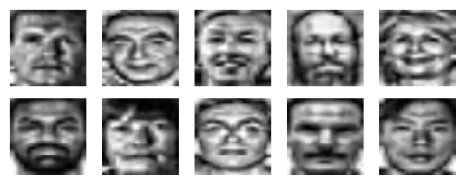
\includegraphics[scale=0.35]{images/faces_overview.png}}
\caption{Overview of the images with faces in the dataset.}
\label{fig:faces-overview}
\end{figure}

\begin{figure}[htbp]
\centerline{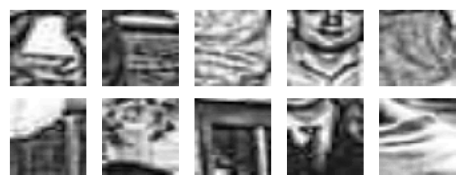
\includegraphics[scale=0.35]{images/non_faces_overview.png}}
\caption{Overview of the images without faces in the dataset.}
\label{fig:non-faces-overview}
\end{figure}

This dataset contains 124 images, 69 of which are face images and 55 are non-face images, with a window of pixels of \(27 \times 18\). We can conclude that the dataset is a little skewed, having more face images than non-face images as it is represented in figure \ref{fig:dataset-distribution}.

\begin{figure}[htbp]
\centerline{
\includegraphics[scale=0.35]{images/data_distribution.png}}
\caption{Analysis of the number of examples for each type of image.}
\label{fig:dataset-distribution}
\end{figure}

\section{Data preprocessing}

\subsection{Resizing and Normalization}
Before applying the classification models we preprocessed our image data. We started off by resizing each image to a window of pixels of \(64 \times 64\), forming a square. Although all the images had the same size before this step, we decided to resize them to a base size that would form a square because it's usually standard procedure in face detection problems.

After this step we validated that each image was in gray-scale, converting from RGB to GRAY and making the problem less complex by having only one dimension to analyze instead of three. We also applied Adaptive Histogram Equalization in the images, so that contrast and luminosity effects were reduced, following the advice and procedure of the authors of the paper \cite{609310}.

To finalize the preprocessing phase, we normalized each image by dividing the pixel values by 255 achieving consistency in all our images, with the pixel values ranging from zero to one.

\subsection{Data Augmentation}
As we stated in section \ref{data-visualization}, the dataset we were given had a total of 124 images. This is an incredibly small dataset and we weren't able to achieve satisfactory results with it, so, we decided to expand the dataset with data augmentation, following some of the practices showcased by the research work explained in \cite{8858529}.

Considering the slight imbalance between the number of examples of face images and non-face images we adopted the following strategy:

\begin{itemize} 
\item Each face image produces 3 new images through reflection and dislocation.
\item Each non-face image produces 4 new images through reflection, dislocation and by inserting a random level of noise.
\end{itemize}

Thereby, ending up with a total of 551 images, 276  of  which  are  face images and 275 are non-face images.

\subsection{Histogram of oriented gradients}
The Histogram of Oriented Gradients (HOG) is a feature descriptor used in computer vision, more specifically in the field of object detection. Instead of our algorithm analysing each image,pixel by pixel, the HOG will count occurrences of gradient orientation in localized portions of an image, improving it's performance. 
Our implementation was based on the example documented in \cite{scikit-hog}, provided by the scikit-image documentation.

\begin{figure}[htbp]
\centerline{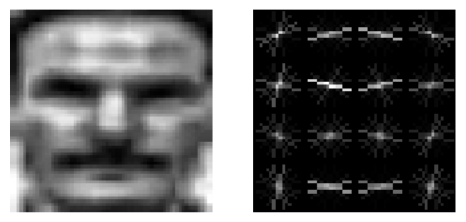
\includegraphics[scale=0.35]{images/hog_image.png}}
\caption{HOG feature extraction}
\label{fig:hog}
\end{figure}

Figure \ref{fig:hog} shows an example of an image before and after applying the Histogram of Oriented Gradients extraction.

\section{Description of the applied machine learning algorithms}

\subsection{Support Vector Machine} \label{svm}

Support Vector Machines (SVM) are highly used due to high empirical performance and somewhat-simple computational complexity, being binary classifiers that when allied with strategies, such as \textit{one-vs-all}, can be expanded to become multi-class classifiers.

In our case, SVM was our first approach to the face detection problem, because the dataset, even after the process of data augmentation, is not very large and we are dealing with a binary classification problem, so we decided to start our initial approach with a simpler model like SVM.

Initially we divide our data in two subsets: training subset with \(80\%\) of the images and testing subset with \(20\%\) of the images.

In SVM there are two main hyper-parameters that can be tweaked to improve the performance of the model, C and Gamma. To get the best performance out of the model we made every combination possible for C and gamma, starting with one of the values present in table \ref{table:svm-initial-configuration}.

\begin{table}[htbp]
\centering
\caption{SVM - Initial Configuration}
\begin{tabular}{ |c|c| } 
 \hline
 \textbf{Train Data} & 80\% \\ 
 \hline
 \textbf{Test Data} & 20\% \\ 
 \hline
 \textbf{Gamma} & [100, 33, 10, 3, 1, 0.3, 0.1, 0.03 ] \\ 
 \hline
 \textbf{C} & [0.01, 0.03, 0.1, 0.3, 1, 3, 10, 30] \\ 
 \hline
\end{tabular}
\label{table:svm-initial-configuration}
\end{table}

To validate which combination of hyper-parameters enabled the best performance out of our model we used K-Fold Cross Validation where our training set was divided in \(K = 5\) smaller sets, where 4 were used for training and 1 was used to validate the model. With this approach we didn't need to reduce the training dataset by creating a validation dataset and the results did not depend on a particular random choice for the pair of (train, validation) datasets.

After validating every combination, as we can see in figure \ref{fig:svm-cross-validation}, the values of C and gamma where our model performed the best are: C = 30 and Gamma = 1.

\begin{figure}[htbp]
\centerline{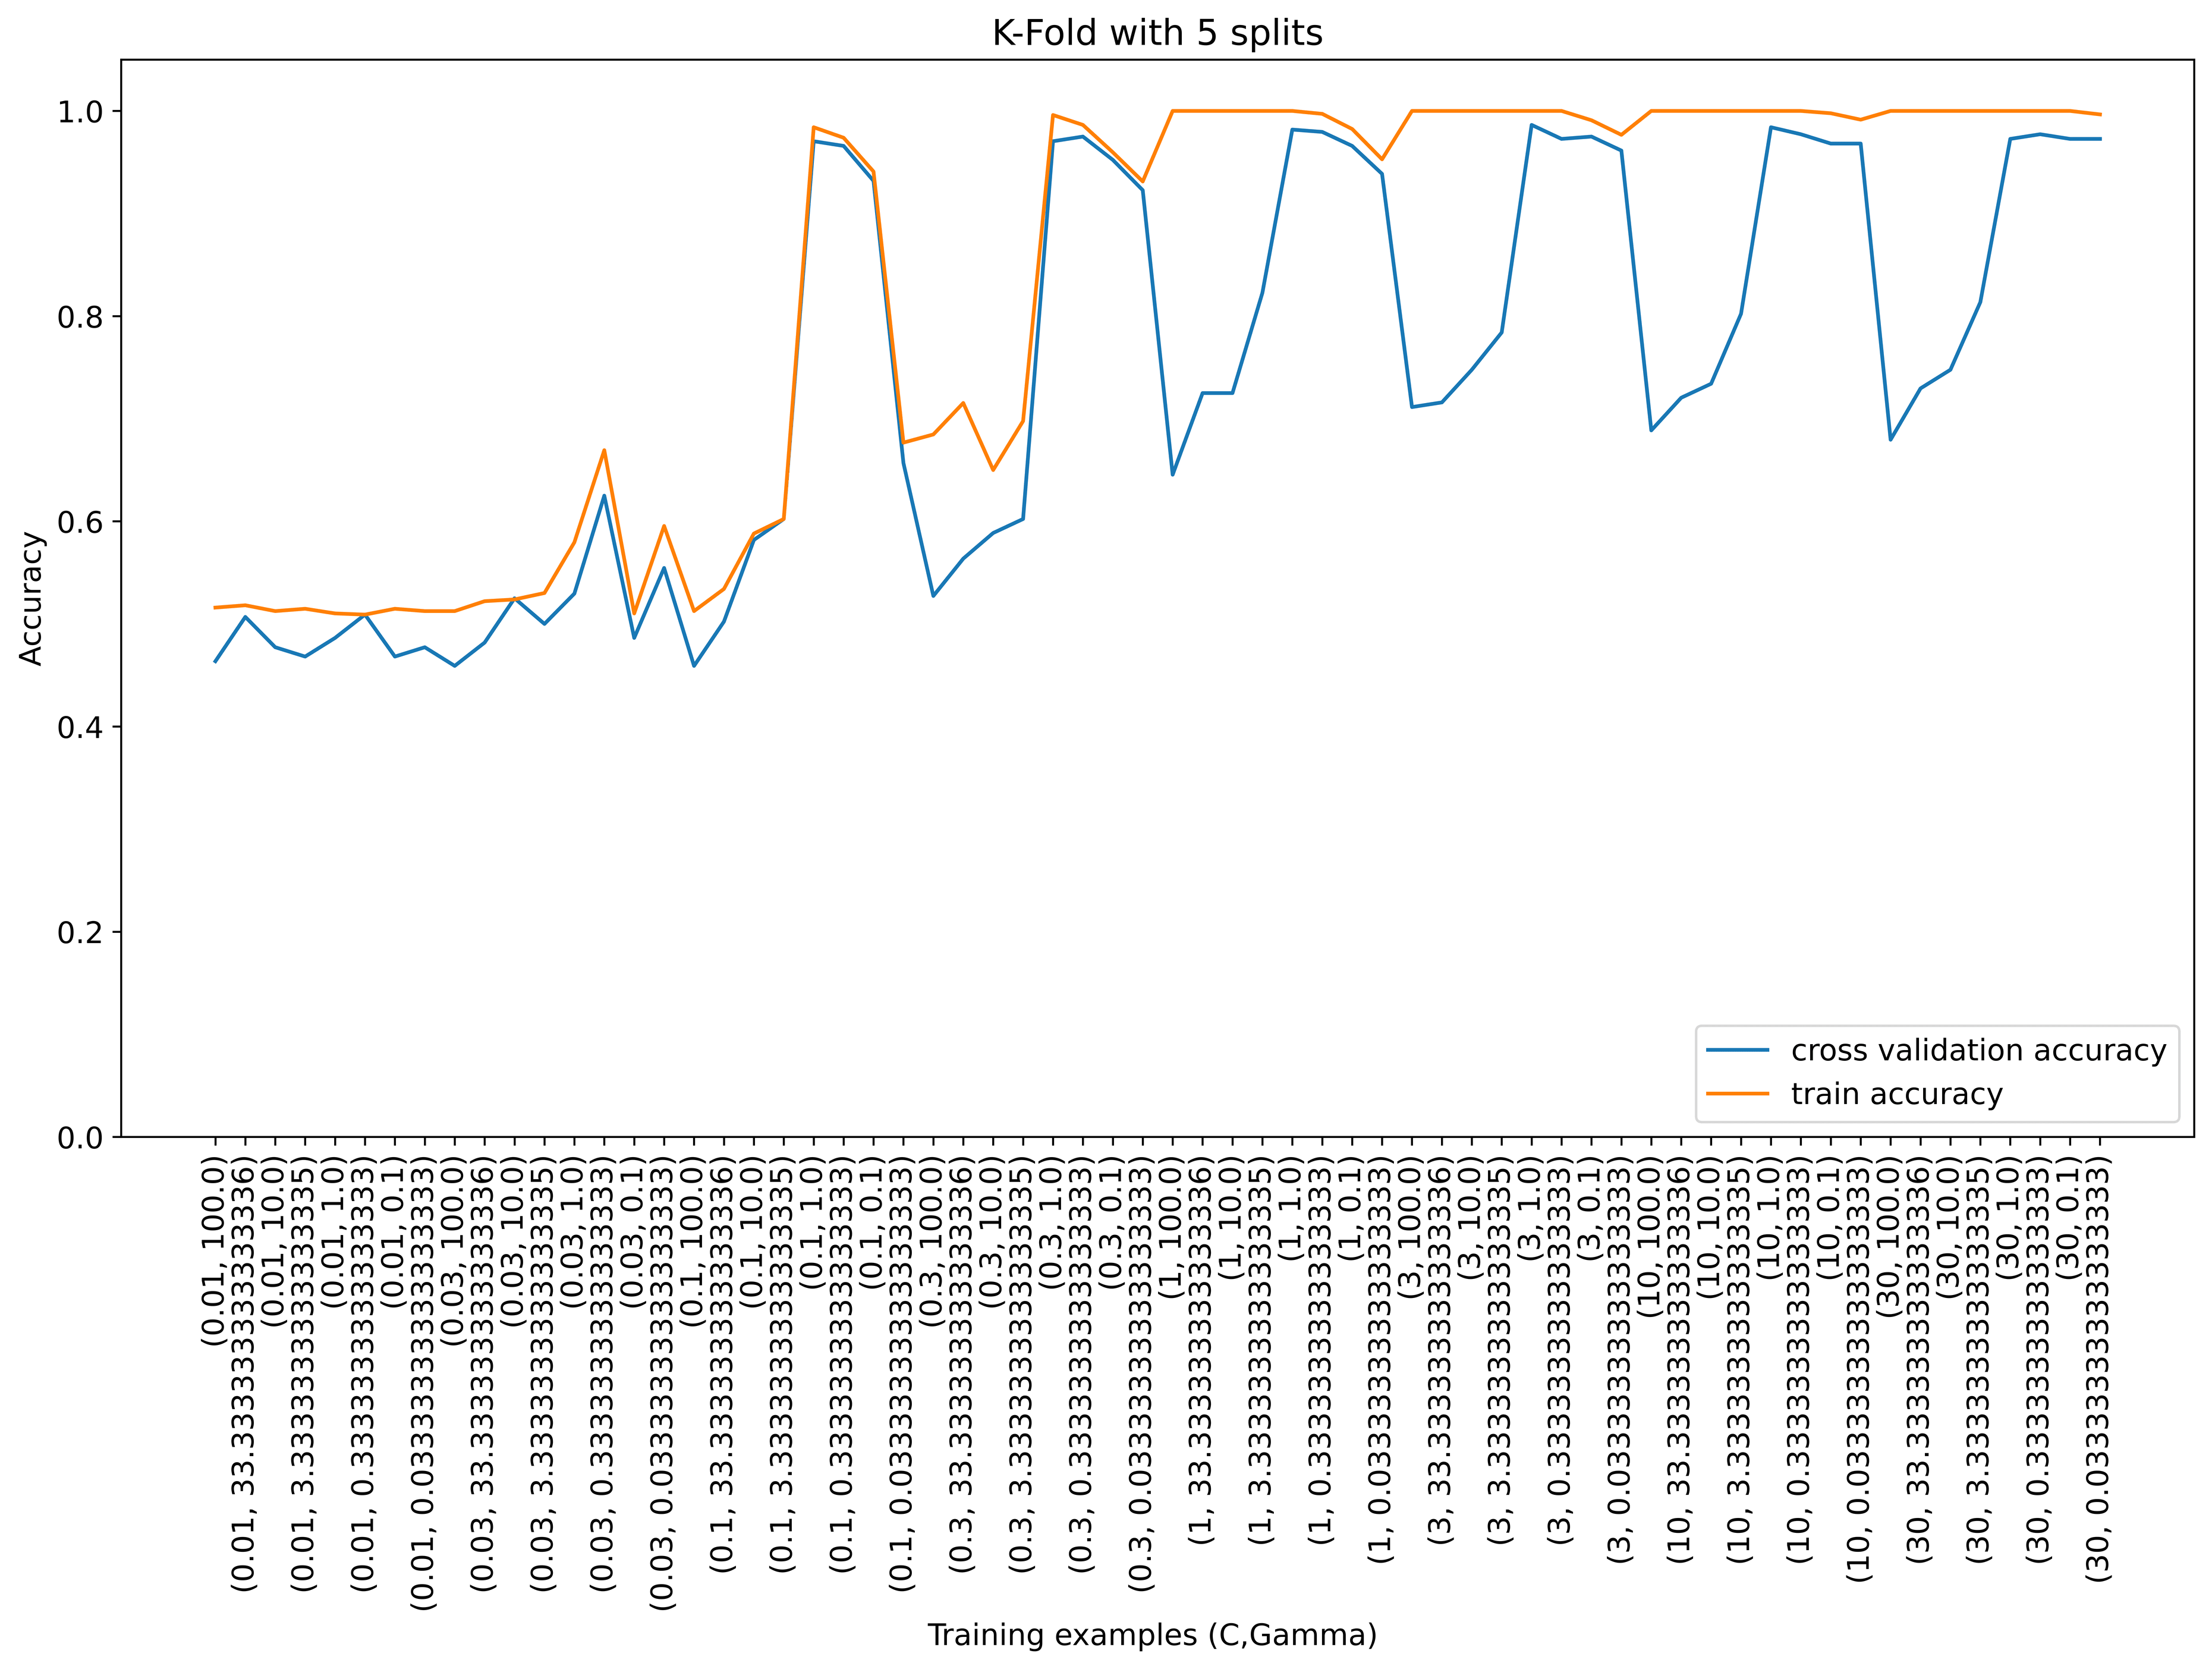
\includegraphics[width=1\linewidth]{images/svm_cross_validation.png}}
\caption{SVM - Cross-Validation using multiple values for C and Gamma}
\label{fig:svm-cross-validation}
\end{figure}

Based on the Cross Validation data, we created an SVM model with a Radial Basis Function (RBF) kernel, and with the hyper-parameters C = 30 and Gamma = 1, that returns 1 when the image is a face, and 0 otherwise, as we can see in table \ref{table:svm-final-configuration}.

\begin{table}[htbp]
\centering
\caption{SVM - Final Configuration}
\begin{tabular}{ |c|c| } 
 \hline
 \textbf{Train Data} & 80\% \\ 
 \hline
 \textbf{Test Data} & 20\% \\ 
 \hline
 \textbf{Kernel} &  Radial Basis Function (RBF) \\ 
 \hline
 \textbf{Gamma} & 1 \\ 
 \hline
 \textbf{C} & 30 \\ 
 \hline
\end{tabular}
\label{table:svm-final-configuration}
\end{table}

Finally, to ensure that the model didn't end up in a local minimum, and that our model was actually learning we run the all process 50 times and calculated the mean values to both train and test phases.


\subsection{Neural Network}

Neural Network (NN) is a classifier that tries to replicate the structure of the human thought.

Being the purpose of the paper to compare the performance of SVM vs NN, our second approach was to implement a Neural Network with a Multi-layer Perceptron Classifier \cite{nn-mlp-classifier}.

Just as in our SVM flow, we initially divide our data in two subsets:

\begin{itemize} 
\item Training subset:  \(80\%\)
\item Testing subset:  \(20\%\).
\end{itemize}


Similar to what was done in SVM, we used HOG as our feature extractor. Hence, the specific implementation we used has 3 layers: \(Input Layer \rightarrow Hidden Layer \rightarrow Output Layer\), with the follow specification:

\begin{itemize} 
\item Input Layer: \(128\) neurons (the respective number of features extracted by HOG);
\item Hidden Layer: \(10\) neurons (as default value, the optimized number of neurons will be specified ahead);
\item Output Layer: \(1\) neuron.
\end{itemize}

Furthermore, we used \textit{RELU} as the activation function, the loss function we used was \textit{Log-Loss Function}, using the \textit{LBFGS} weight optimizer (we decide to use \textit{LBFGS}, because, according to Scikit-Learn documentation \cite{nn-mlp-classifier}, it can converge faster and perform better, given smaller datasets, which is our case), and has the default learning rate, we used \( \alpha = 0.001 \), which will be optimized further ahead. To summarize we can see the initial configuration of our Neural Network in table \ref{table:nn-initial-configuration}.

\begin{table}[htbp]
\centering
\caption{NN - Initial Configuration}
\begin{tabular}{ |c|c| } 
 \hline
 \textbf{Train Data} & 80\% \\ 
 \hline
 \textbf{Test Data} & 20\% \\ 
 \hline
 \textbf{Input Layer} & \(128\) neurons \\ 
 \hline
 \textbf{Hidden Layer} & [10, 20, 30, 40, 50, 60, 70] neurons, \(default = 10\) \\ 
 \hline
 \textbf{Output Layer} & \(1\) neuron \\ 
 \hline
 \textbf{Activation Function} & \textit{RELU} \\ 
 \hline
 \textbf{Loss Function} & \textit{Log-Loss Function}, via \textit{LBFGS} weight optimizer \\ 
 \hline
 \textbf{Learning Rate (\(\alpha\))} & [0.001, 0.01, 0.05, 0.1, 0.5, 1, 10], \(default = 0.001\) \\ 
 \hline
 \textbf{Number of Iterations} & [100, 200, 300, ..., 900, 1000], \(default = 100\) \\ 
 \hline
\end{tabular}
\label{table:nn-initial-configuration}
\end{table}

As done in the previous section, the SVM aproach \ref{svm}, we optimized the hyper-parameters of the NN model to enable its best performance. Just like in SVM, we did this by applying K-Fold Cross Validation, with \(K = 5\). The hyper-parameters we decided to vary, and consequently optimize, were as follows:

\begin{itemize} 
\item Hidden Layer size (the number of neurons in the Hidden Layer);
\item Learning rate (\(\alpha\));
\item Number of iterations.
\end{itemize}

After validating every combination, as we can see in figure \ref{fig:nn-cross-validation}, our model performed the best when:

\begin{itemize} 
\item \( HiddenLayerSize = 60 \) neurons;
\item \( \alpha = 1 \);
\item \( NumberOfIterations = 700 \).
\end{itemize}

\begin{figure}[htbp]
\centerline{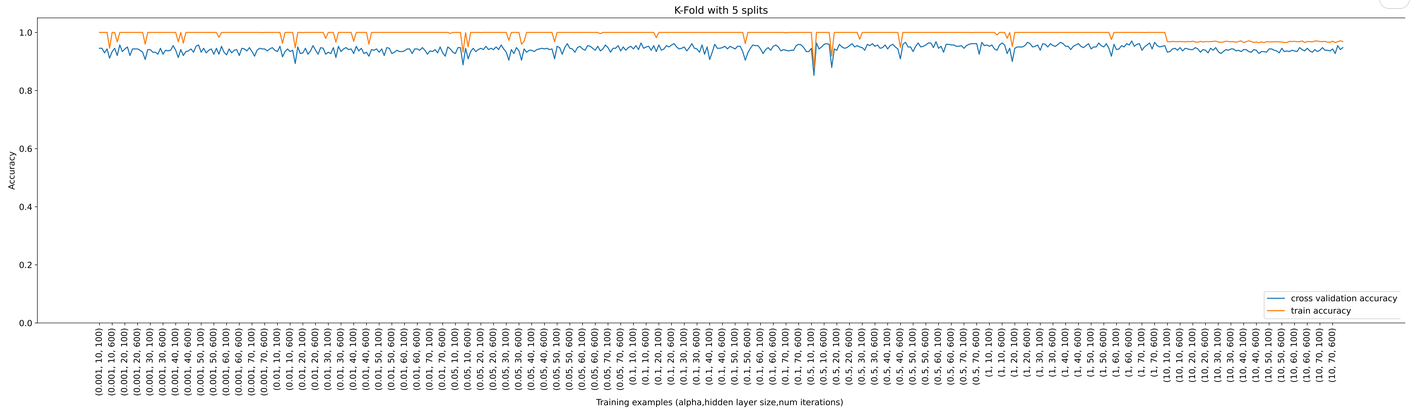
\includegraphics[width=1\linewidth]{images/nn_cross_validation.png}}
\caption{NN - Cross-Validation using multiple-value combinations}
\label{fig:nn-cross-validation}
\end{figure}

Based on the Cross Validation data, we created a Neural Network with a Multi-layer Perceptron Classifier, and a final configuration that can be seen in table \ref{table:nn-final-configuration}.

\begin{table}[htbp]
\centering
\caption{NN - Final Configuration}
\begin{tabular}{ |c|c| } 
 \hline
 \textbf{Train Data} & 80\% \\ 
 \hline
 \textbf{Test Data} & 20\% \\ 
 \hline
 \textbf{Input Layer} & \(128\) neurons \\ 
 \hline
 \textbf{Hidden Layer} & \(60\) neurons \\ 
 \hline
 \textbf{Output Layer} & \(1\) neuron \\ 
 \hline
 \textbf{Activation Function} & \textit{RELU} \\ 
 \hline
 \textbf{Loss Function} & \textit{Log-Loss Function}, via \textit{LBFGS} \\ 
 \hline
 \textbf{Learning Rate (\(\alpha\))} & \(\alpha = 1\) \\ 
 \hline
 \textbf{Number of Iterations} & 700 \\ 
 \hline
\end{tabular}
\label{table:nn-final-configuration}
\end{table}

Finally, and as we did in our SVM approach, to ensure that the model didn't end up in a local minimum, and that our model was actually learning we run the all process 50 times and calculated the mean values to both train and test phases.

\section{Results and Discussion} \label{section:results}
In this chapter are presented some scenarios and tests with extreme value changes to better understand how the market could evolve in the near future and is also very useful to detect flaws in the model.

\subsection{Basic scenario}
The basic scenario is based on the values explained throughout section \ref{section:model}. Figure \ref{fig:adopters} shows an exponential growth of the population of adopters, characterized by a slow
but steady growth in the beginning (year 2020-2027), and a large growth in the end (year 2028-
2040). In figure \ref{fig:adoption-rate} can also be seen the adoption rate with an exponential behavior, especially in the first 15 years. Both results are obviously connected, by the model definition, and this exponential growth is due to the fact that, as seen earlier, most of the factors are in the acceptable conditions "imposed" by the customers after the first 10 years, meaning that after those 10 years (in 2030) the consumers start more easily and frequently purchasing electric vehicles, hence, the exponential growth.

\begin{figure}[htbp]
\centering
\begin{subfigure}{0.55\textwidth}
  \centering
  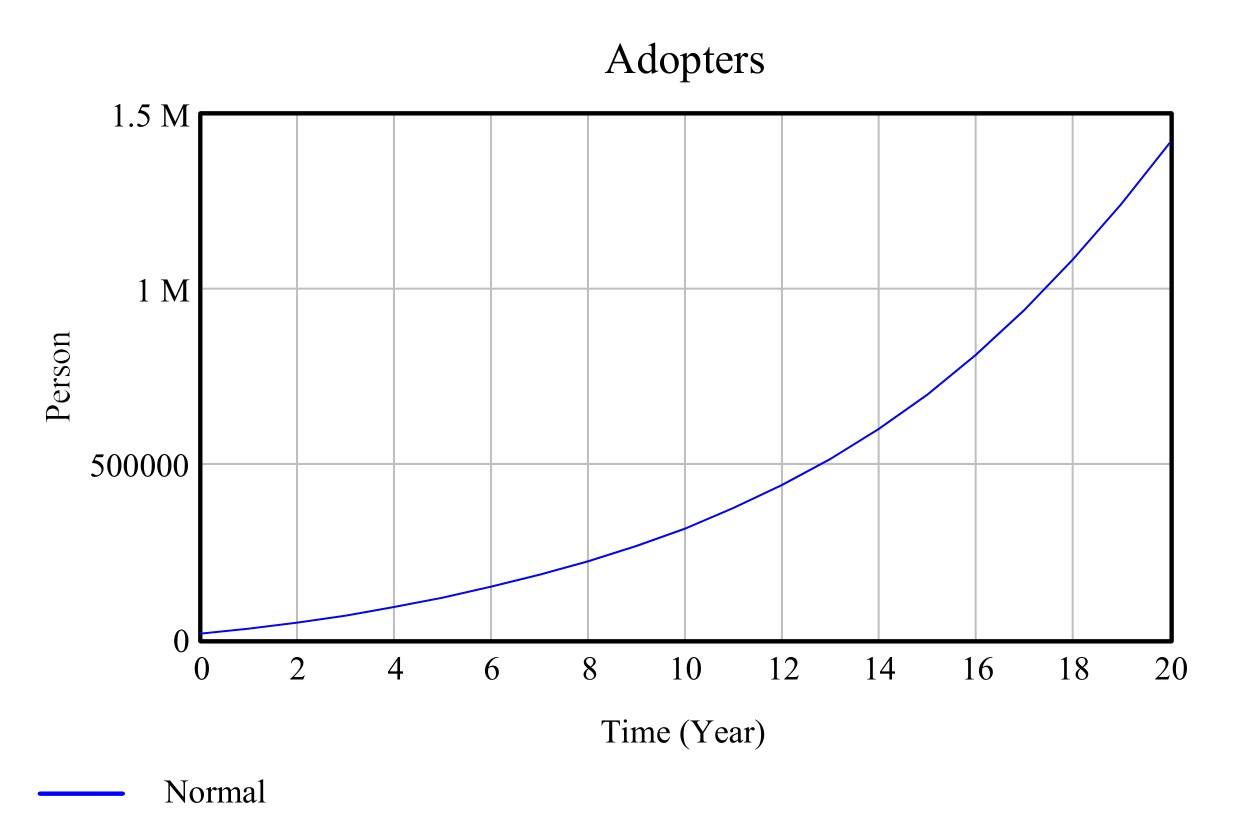
\includegraphics[width=0.98\linewidth]{img/results-basic.jpg}
  \caption{Adopters growth/evolution over the years}
  \label{fig:adopters}
\end{subfigure}%
\begin{subfigure}{0.45\textwidth}
  \centering
  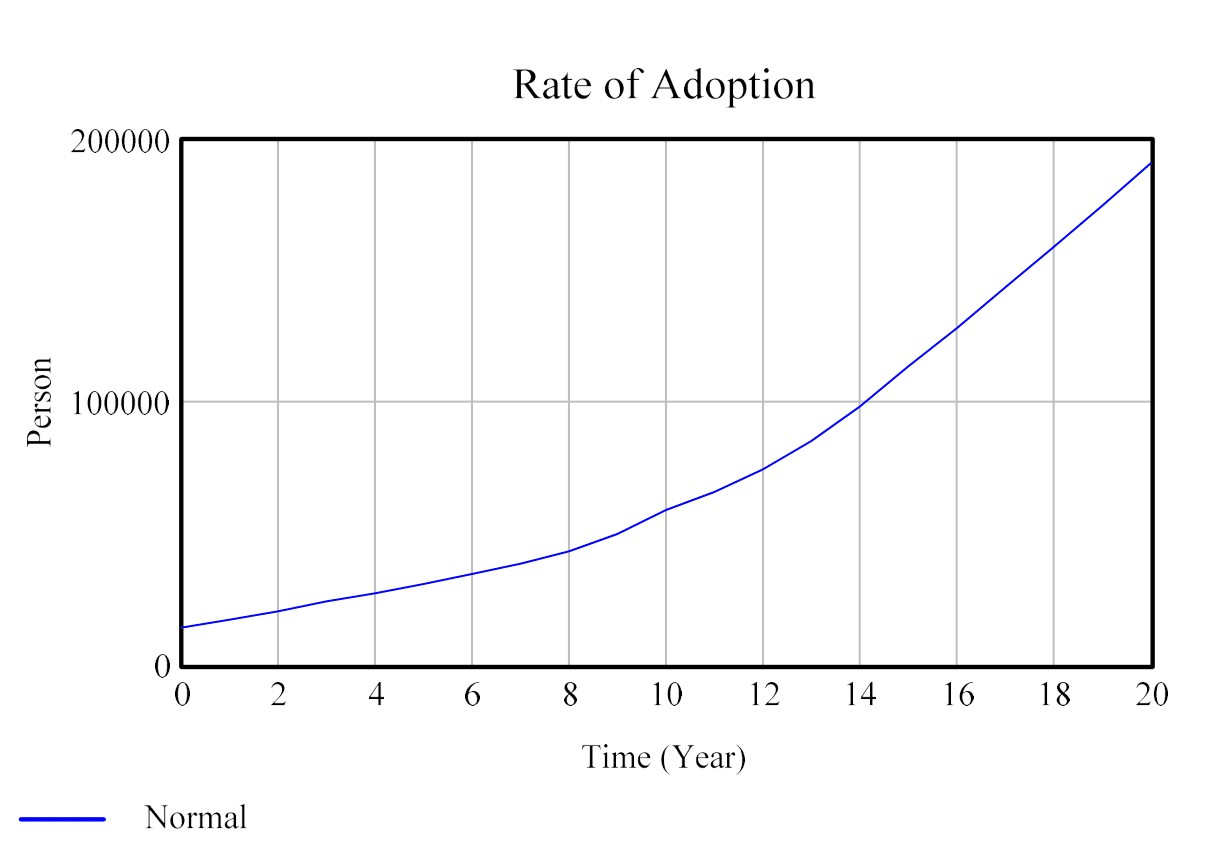
\includegraphics[width=0.98\linewidth]{img/results-basic-adoption-rate.jpg}
  \caption{Rate of Adoption over the years}
  \label{fig:adoption-rate}
\end{subfigure}
\caption{Graphical representation of basic scenario results}
\label{fig:basic-scenario}
\end{figure}

\subsection{Scenario Situations}
Scenario situations use the same values for the model as in the basic situation except from the variable that is being tested or changed to simulate a particular scenario and are useful to create insights for the model and to make the assumptions more reliable.

\subsubsection{Price Difference Effect}
The price difference between an EV and an ICV is the most crucial factor that keeps potential adopters from purchasing an EV. According to the surveys and the information portrayed in section \ref{section:model}, the area around a zero (or negative) price difference has the most effect on the adopters. In contrast to others factors such as driving range, the price difference can be "artificially" influenced through subsidies given by the government. Therefore the subsidy scenario is given in a situation where the government would provide a subsidy of 5000\euro \space on the vehicle fixed price from 2020 to 2029, that is, the first 9 years.

\begin{figure}[htbp]
\centerline{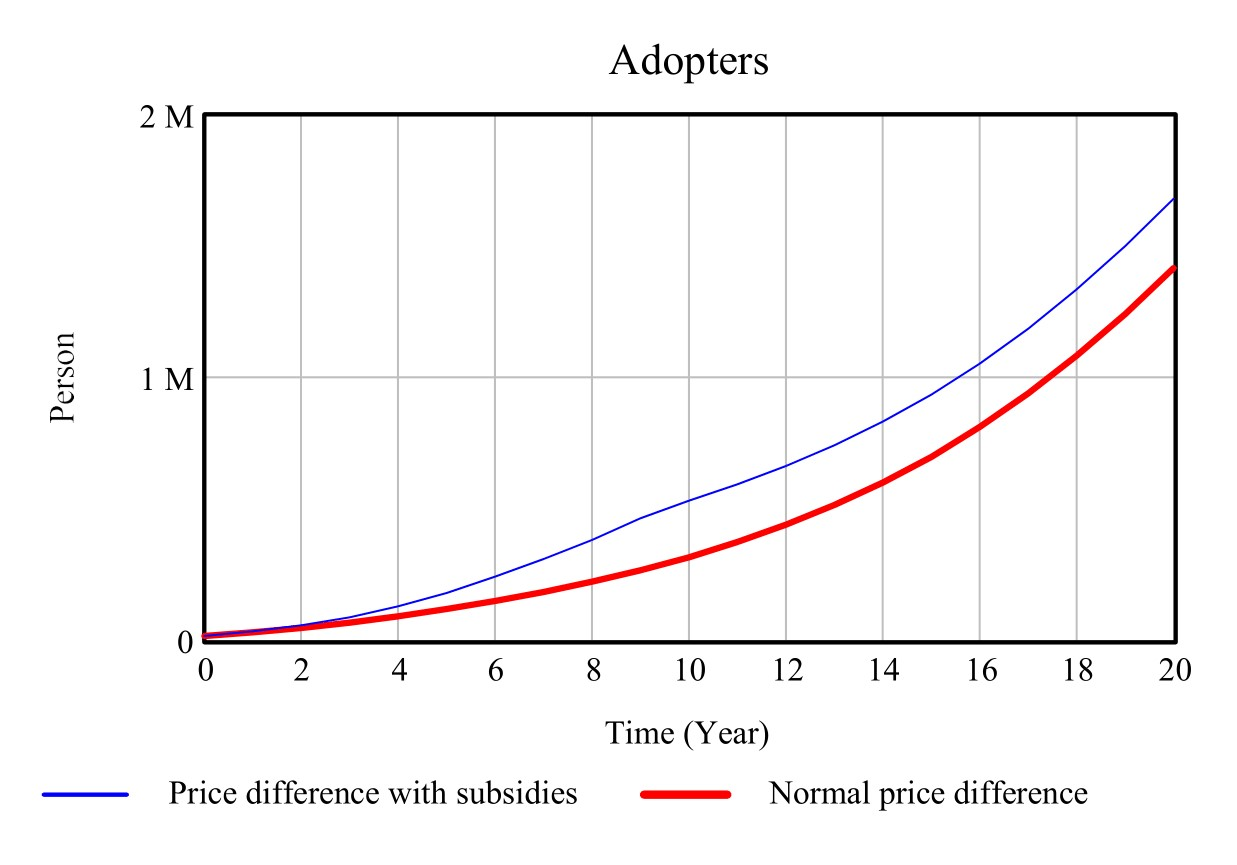
\includegraphics[width=0.7\linewidth]{img/results-price-difference.jpg}}
\caption{Adopters Growth in function of Price Difference variations}
\label{fig:results-price-difference}
\end{figure}

Figure \ref{fig:results-price-difference} shows the result of the scenario described above. As we can see in the graph, the subsidy allowance was effective in the sense that in the first 9 years, the adoption rate clearly increased because in the same time-frame the scenario with the subsidies had a bigger growth of adopters than the basic one. After those 9 years, the adoption rate decreases a little and approximates to the adoption rate of the basic scenario. This "boost" on the first 9 years was able to positively influence the EV market as we ended the 20-year time-frame with considerably more EV adopters in the altered scenario when compared to the basic one. 

\subsubsection{Infrastructure Network Density and Recharge Time Effect}
In this section, the study focuses on the infrastructure network density and the recharge time effects on the EV market.

In this verification, there are 3 different scenarios: \textbf{the normal one}, \textbf{the scenario with a high density infrastructure and slow charging times} and one last \textbf{scenario with a high density infrastructure and fast charging capabilities}. The normal one is the basic scenario referenced earlier.

The other two scenarios have a high density recharging network, meaning that we have total coverage on Portuguese territory from the start (year 2020). The graph of the actual recharge network density in these scenarios has a similar appearance/behaviour to the normal one, being the only difference the starting value that in these scenario has a value of density of 10km, instead of 100km.

What sets these two scenarios apart is the charging times, in one of them, we have slow charging capabilities (with a initial value of 8 hours) and in the other we have fast charging capabilities (with a initial value of 30 minutes).

The time range is set to 10 years, because this better shows the effect of the infrastructure and recharging times in the early phase of the adoption process.

\begin{figure}[htbp]
\centerline{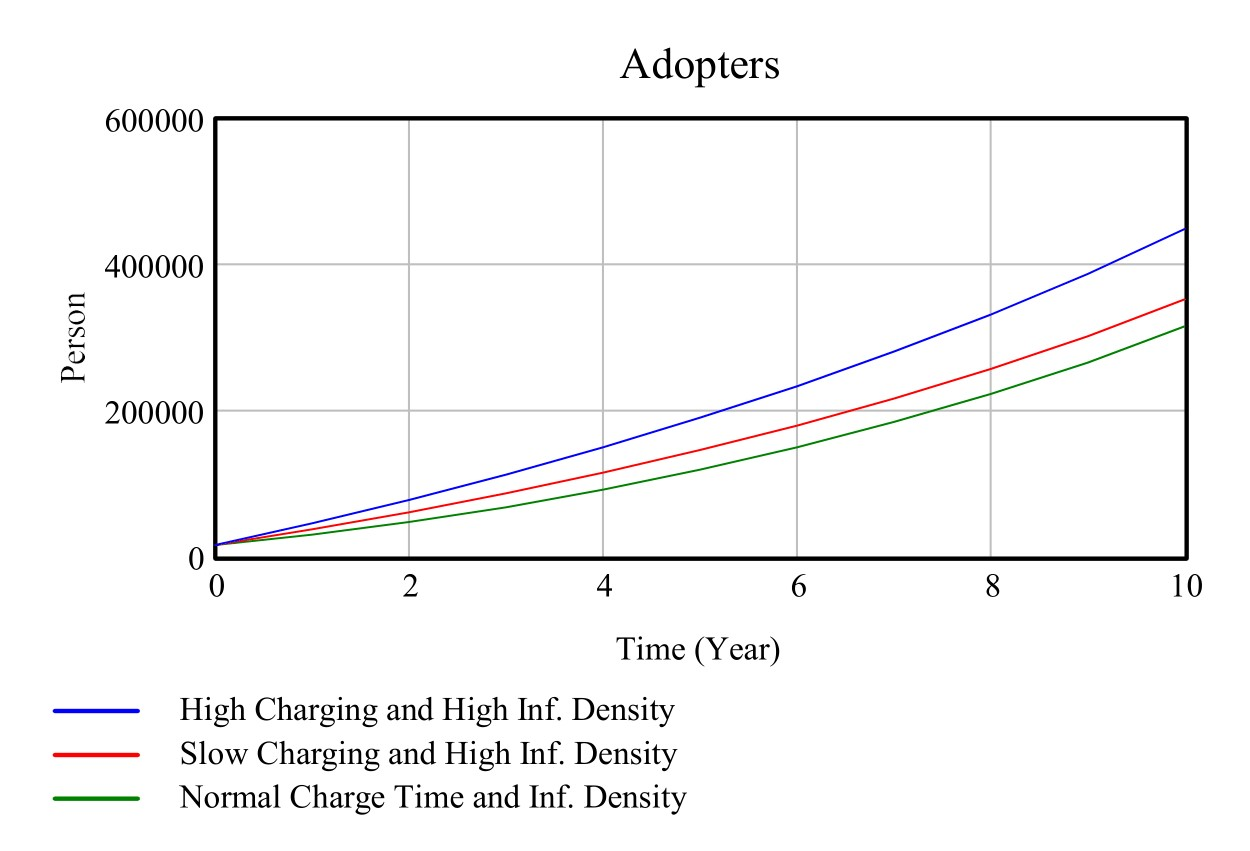
\includegraphics[width=0.7\linewidth]{img/results-time-and-density.jpg}}
\caption{Adopters Growth in function of Infrastructure Density and Charging Time variations}
\label{fig:results-time-and-density}
\end{figure}

Figure \ref{fig:results-time-and-density} shows the result of the scenario described above. As we can see in the graph, these scenario simulations allows us to conclude that the population of adopters increases as result of both \textbf{high infrastructure density} and \textbf{fast charging capabilities}. As we can see, the scenario with high recharge infrastructure density and slow charging is still able to "produce" more adopters than the basic scenario. This is related with the premised stated earlier that a high density recharge network allows for slower charging times, because there is high availability of charging stations. The optimal scenario is when we have a high density charging infrastructure and fast charging capabilities from the start, being these two conditions the best of both worlds. However, a optimistic yet feasible scenario is to have a high density charging network in the early stages of EV introduction (first 10-15 years) and then focusing on improve the charging times of the already existent EV charging stations.

\clearpage

\section{Novelty and contributions} \label{novelty}

In view of the analyzed papers and research work, although not all are using the same data (since we didn't find any papers using the same dataset we used), we consider to have not made any novelty or contributions regarding our work, as we kept very close to what has been done in the context of face detection. However, considering the topics we will discuss next, we consider to have owned some positive impact regarding the success rate of the face detection system. 

The next analysis will be made taking into consideration that none of the found research work used the same dataset we did, so most of our comparisons are not totally representative of what may be the reality, but are an indication of what we were able to achieve in comparison to other's work, given our dataset.

\subsection{Support Vector Machine (SVM)}
Regarding the SVM classifier, in the work present in \cite{1619082} the authors stated an accuracy of \(95\%\), in the paper in \cite{609310} the authors stated an accuracy of \(97.1\%\) and in the study in \cite{5076875} the authors stated an accuracy of \(94.7\%\). Considering that we were able to achieve an F1 Score, Precision, Recall an Accuracy of approximately \(98.5\%\), we can conclude that our SVM classifier is better and more accurate than the ones in these papers.  We can also say that, being our model \(1.4\%\) more effective than the best model in the reseach found, we were able to give a little contribution to this field providing a more effective and accurate SVM-based solution to problem of face detection. 

\subsection{Neural Network (NN)}
Regarding the NN classifier, in the work present in \cite{5233453} the authors stated an accuracy of \(91.43\%\) and in the study in \cite{8858529} the authors stated an accuracy of \(96.24\%\). Considering that were able to achieve an F1 Score, Precision, Recall an Accuracy of approximately \(97.3\%\), although not a perfect result we were mostly satisfied with this outcome as we based some of our approach \cite{5233453} and were able to outperform it. The approach described in the work present in \cite{8858529} was based on a CNN and it was done with a much larger dataset than the one we used, so, we cannot compare our results with theirs. 

Finally, based on some papers and online notebooks, we think that as future work to optimize and improve our NN-based application we could benefit from the usage of Fast Gabor Filtering as our feature extractor. Another possible improvement would be to use a combination between a skin-color segmentation algorithm (to choose candidate areas with the use of other masks on top of the skin-color segmentation) with the use of a candidate area re-scaling algorithm, to make possible to detect faces with sizes different than \(27 \times  18\), as detailed in \cite{5076875}.

\section{Conclusion}
All in all, we are satisfied with the models we were able to develop. We also realized that, in some notion, we managed to contribute to improve the current state of the art of an SVM-based application on face detection and, even though, or NN-based classifier did not achieve what we initially expected we also managed to present an increment in accuracy and effectiveness comparing to the research found on this topic.

Finally, we can also conclude that our SVM-based application with HOG as a feature extractor is pretty viable  to be used in real world scenarios where we need a model that is able to quickly detect faces, even if some times produces some false positive results.

\section*{Work Done By Each Student}
Due to the restrictions of Covid-19 virus, we were not able to always develop the project together (in the same place or close to each other).

Therefore, João Vasconcelos was responsible for the implementation of Feature Extraction (HOG) and the Neural Network and Vasco Ramos was responsible for the topic of Data Augmentation and Support Vector Machines.

Overall, we consider the work was split equally between both members.

To summarize:

\begin{itemize} 
\item João Vasconcelos (50\%) - Feature Extraction (HOG), Train/test NN and Papper.
\item Vasco Ramos (50\%) - Data Augmentation, Train/test SVM and Papper.
\end{itemize}

\bibliography{refs}
\bibliographystyle{ieeetr}

\end{document}
